\subsection{Andrew Nielsen}

I'm working towards getting my Masters degree in Cybersecurity. My goal for this course is to be able to prepare for my PhD down the road and be able to apply the research knowledge I gain from this class herein. I'm hoping to learn how to read efficiently and quickly navigate through research documents. I'm looking to be able to understand how to research and how to narrow down a topic that will help in the future. I'm studying cybersecurity in the master's program. 

The research area that I have been working on is ransomware with fuzzy techniques in geo-spatial systems. Part of it has been in understanding ransomware, fuzzing, and identifying gaps in geo-spatial research extending past the earth's atmosphere.

Some code that I found on GitHub that deals with ransomware was found \href{https://github.com/mauri870/ransomware.git}{here}. This code actually simulates how ransomware behaves and encrypts all the files on a machine and stores the encryption key on a remote server so the user is not able to decrypt their files. I did not have to deal with any merge conflicts when updating files and committing them back to the repository.


A picture of myself can be seen below:

\begin{figure}[htp]\centering
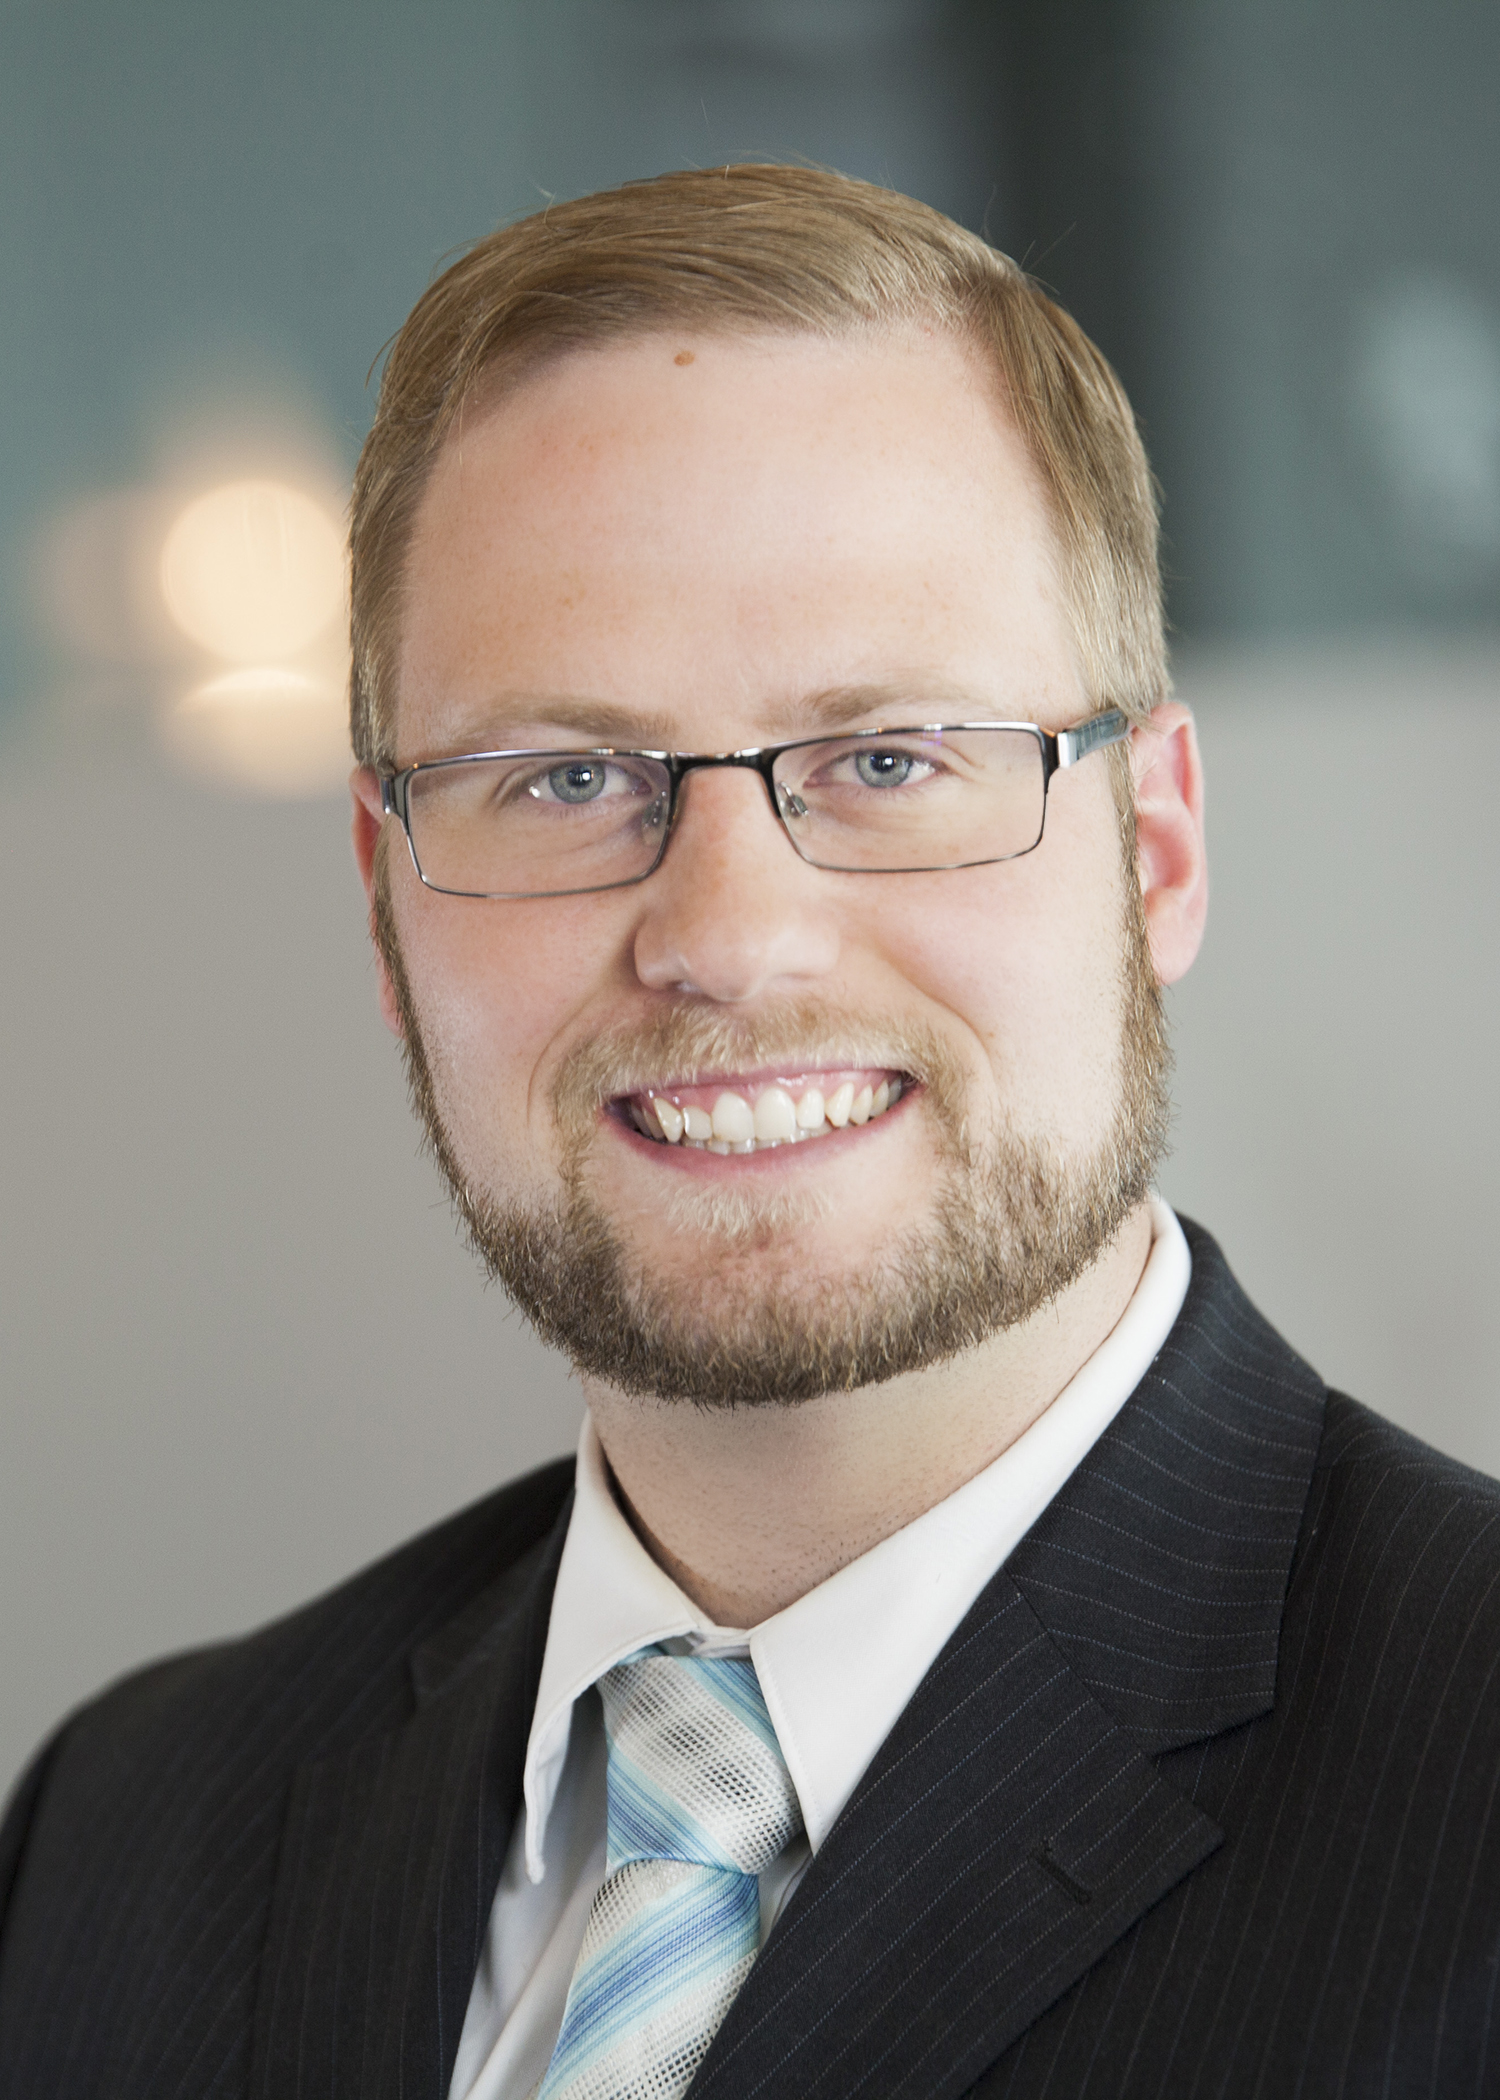
\includegraphics[width=.3\textwidth]{Andrew Professional picture.jpg}
\caption{Andrew Nielsen's Picture}
\label{fig:Andrew Professional picture}
\end{figure}

\subsubsection{QA}

\begin{enumerate}
    \item WW: Where did you do your undergrad?

	AN: I did my undergrad at Weber State University in Accounting and Information Systems and Technology. 

    \item DH: How soon are you looking to start your PhD? Directly after your Master's?

	AN: The more I think about it the more that I want to wait as the work i'm currently doing doesn't line up to much with research. It may not be until kids are out of the house. haha
\end{enumerate}

